\section{Evaluation}
\label{sec:evaluation}

In this section we present a quantitative evaluation \textit{for two corpus} of the algorithm proposed in this paper \textit{and a comparative evaluation}. In the GRE area there was a common assumption that there is a gold standard ordering for a given domain~\cite{Dale1995}. However, this assumption has been dropped after empirical studies such as those presented in~\cite{arec2:2008:Areces,viet:gene11}. It has been observed that not only there is no single ordering of properties that covers all human-produced descriptions in a given domain but, in fact, it is not even the case that each speaker consistently uses just one ordering. In this section we show that the probabilistic algorithm presented in the previous section is able to generate a distribution of REs similar to that observed in corpora, even when no corpus specific for a target object is available. 


\subsection{Evaluation of the GRE3D7}
%\label{sec:evaluacionGRE3D7}

\textit{A quantitative evaluation over the GRE3D7}. Using \puse~learned as described in Section~\ref{sec:learning} and running our algorithm 10000 times, we obtain 14 different referring expressions for Figure~\ref{GRE3D7-stimulus}. The algorithm generates 5 of the 12 different kinds of REs observed in the 140 occurrences of the corpora. We also generate other 9 REs for the target, not present in the corpora, but natural sounding as can be observed in Table~\ref{results-algo-fig3} that only represent a 1,52\% of the utterances generated by the algorithm. Hence, 98,48\% of the utterances generated by the algorithm appear in the corpora. In the table we list all the REs found in the corpus for Figure~\ref{GRE3D7-stimulus} and all the RE generated by our algorithm using the learned \puse. For each RE, we indicate the number of times it appears in the corpus (\#Cor), the proportion of the corpus its frequency represents (\%Cor), the number of times it is generated by our algorithm (\#Alg) and the proportion of the generated REs its frequency represents (\%Alg). Finally, the accuracy (\%Acc) column compares the REs in the corpus with respect to the REs generated by the algorithm. The accuracy is the proportion of perfect matches between the algorithm output and the human REs from the corpus. The accuracy metric has been used in previous work for comparing the output of a REG algorithm with the REs found in corpora~\cite{sluis07:eval,viet:gene11} and is considered an strict comparison metric for this task. 

\begin{table}[h!]

\begin{center}
\begin{tabular}{|l|c|c|c|c|c|}
\hline
RE & \#Cor & \%Cor & \#Alg & \%Alg & \%Acc \\
\hline
ball,green & 91 & 65 & 6376 & 63,76 & 63,76 \\
ball,green,small & 23 & 16,43 & 3440 & 34,40 & 16,43 \\
ball,green,small,on-top(blue,cube,large) & 8 & 5,71 & 0 & 0 & 0 \\
ball,green,on-top(blue,cube) & 5 & 3,57 & 0 & 0 & 0 \\
ball,green,on-top(blue,cube,large) & 5 & 3,57 & 0 & 0 & 0 \\
ball,green,small,on-top(blue,cube) & 2 & 1,43 & 0 & 0 & 0 \\
ball,on-top(cube) & 1 & 0,71 & 27 & 0,27 & 0,27 \\
ball,green,small,on-top(blue,cube,large,left) & 1 & 0,71 & 0 & 0 & 0 \\
ball,small,on-top(cube,large)	& 1 & 0,71 & 2 & 0,02 & 0,02 \\
ball,green,top & 1 & 0,71 &	0 & 0 & 0 \\
ball,small,on-top(cube) & 1 & 0,71 & 3 & 0,03 & 0,03 \\
ball,green,on-top(cube) & 1 & 0,71 & 0 & 0 & 0 \\
ball,front,green & 0 & 0 & 97 & 0,97 & 0 \\
ball,front,green,small & 0 & 0 & 13 & 0,13 & 0 \\
ball,front,top & 0 & 0 & 12 & 0,12 & 0 \\
ball,green,left	& 0 & 0 & 11 & 0,11 & 0 \\
%ball,on-top(blue,cube) & 0 & 0 & 32 & 0,32 & 0 \\
ball,top & 0 & 0 & 10 & 0,10 & 0 \\
ball,green,left,small & 0 & 0 & 5 & 0,05 & 0 \\
ball,left,top & 0 & 0 & 2 & 0,02 & 0 \\
ball,small,top & 0 & 0 & 1 & 0,01 & 0 \\
ball,front,on-top(cube,left) & 0 & 0 & 1 & 0,01 & 0 \\
%ball,green,small,on-top & 0 & 0 & 14 & 0,14 & 0 \\
%ball,green,left,on-top(blue,cube),small & 0 &  0 & 7 & 0,07 & 0 \\
\hline
Total & 140 & 100 & 10000 & 100 & 80,51 \\
\hline
\end{tabular}
\caption{Referring expressions produced by the algorithm for Figure~\ref{GRE3D7-stimulus}\label{results-algo-fig3}}
\end{center}
\end{table}

In order to put our results in perspective we compare the accuracy obtained for \textit{all} figures in the corpus using the probability of used inferred (column Learned \puse) and the probability of used directly extracted from corpora (column Model \puse) as explained in Section~\ref{sec:learning}. We show the accuracy results in Table~\ref{results-algo-all}. The random baseline (column Random) is calculated in by producing random probabilities of use and then running the algorithm 10000 using these random probabilities. Not only the intersection between the randomly generated REs and the corpus is lower but also many of  the REs generated in this way are not naturally sounding (e.g. ``small on the top of a blue cube that is below of something that is small''). We also show the results of accuracy for uniform distribution (column Uniform) as a second baseline. We calculate the uniform distribution by assigning each RE generated by the algorithm or in corpora the same proportion. 

\begin{table}[h!]
\begin{center}
\begin{tabular}{|l|c|c|c|c|}
\hline
Figure & Model \puse &  Learning \puse & Random \puse &  Uniform \puse \\
\hline

Fig. 1	&	89,29\%	&	85,62\%	&	24,75\%	&	0.00\\%	\\
Fig. 2	&	73,28\%	&	63,66\%	&	6,99\%	&	0.00\\%	\\
Fig. 3	&	82,93\%	&	81,53\%	&	3,61\%	&	0.00\\%	\\
Fig. 4	&	69,41\%	&	73,73\%	&	1,37\%	&	0.00\\%	\\
Fig. 5	&	90,65\%	&	51,59\%	&	0,13\%	&	0.00\\%	\\
Fig. 6	&	87,24\%	&	80,35\%	&	4,35\%	&	0.00\\%	\\
Fig. 7	&	84,25\%	&	51,26\%	&	5,19\%	&	0.00\\%	\\
Fig. 8	&	80,94\%	&	72,92\%	&	4,39\%	&	0.00\\%	\\
Fig. 9	&	90,89\%	&	70,33\%	&	0,87\%	&	0.00\\%	\\
Fig. 10	&	91,31\%	&	73,96\%	&	8,75\%	&	0.00\\%	\\
Fig. 11	&	80,64\%	&	58,76\%	&	0,36\%	&	0.00\\%	\\
Fig. 12	&	77,16\%	&	76,06\%	&	0,2\%	&	0.00\\%	\\
Fig. 13	&	91,18\%	&	49,87\%	&	1,44\%	&	0.00\\%	\\
Fig. 14	&	94,44\%	&	68,7\%	&	1,35\%	&	0.00\\%	\\
Fig. 15	&	85,07\%	&	46,49\%	&	3,14\%	&	0.00\\%	\\
Fig. 16	&	82,4\%	&	61,79\%	&	0,52\%	&	0.00\\%	\\
Fig. 17	&	92,65\%	&	86,59\%	&	6,92\%	&	0.00\\%	\\
Fig. 18	&	90,24\%	&	77,34\%	&	31,66\%	&	0.00\\%	\\
Fig. 19	&	90,83\%	&	78,73\%	&	0,2\%	&	0.00\\%	\\
Fig. 20	&	83,65\%	&	67,48\%	&	1,79\%	&	0.00\\%	\\
Fig. 21	&	92,81\%	&	83,47\%	&	2,77\%	&	0.00\\%	\\
Fig. 22	&	88,34\%	&	83,05\%	&	1,56\%	&	0.00\\%	\\
Fig. 23	&	85,92\%	&	71,11\%	&	0,73\%	&	0.00\\%	\\
Fig. 24	&	89,86\%	&	79,37\%	&	1,98\%	&	0.00\\%	\\
Fig. 25	&	86,33\%	&	70,05\%	&	11,97\%	&	0.00\\%	\\
Fig. 26	&	86,52\%	&	71,98\%	&	15,58\%	&	0.00\\%	\\
Fig. 27	&	71,59\%	&	67,78\%	&	2,79\%	&	0.00\\%	\\
Fig. 28	&	78,4\%	&	77,13\%	&	1,6\%	&	0.00\\%	\\
Fig. 29	&	92,36\%	&	73,83\%	&	1,78\%	&	0.00\\%	\\
Fig. 30	&	89,64\%	&	70,41\%	&	38,83\%	&	0.00\\%	\\
Fig. 31	&	85,85\%	&	70,98\%	&	0,88\%	&	0.00\\%	\\
Fig. 32	&	86,46\%	&	73,11\%	&	5,68\%	&	0.00\\%	\\
\hline
Average	&	85.7\%	&	70.91\%	&	6.07\%	&	0.00\%	\\

\hline
\end{tabular}
\caption{Percentage on intersection between the REs generated using directly extracted from the figure corpora\label{results-algo-all}, learned probabilities, random and uniform probabilities}
\end{center}
\end{table}

The table shows that the accuracy is not stable for all scenes, ranging from 86.59\% in Fig. 17 to 46.49\% in Fig. 15. The drop in accuracy that we see for Fig 15 is due to the characteristic of the behavior of size in the domain that we were not able to capture and that we discussed in Section~\ref{sec:learning}. 

To show the results from a different perspective than that of accuracy we also compute the cross-entropy~\cite{juraksky:spee08} between the corpus distribution of REs and each algorithm (the Model, the Learned, and the two baselines).    

%The entropy a measure of the amount of uncertainty associated with the value of the variable. The cross entropy between two probability distributions measures the average number of bits needed to identify an event from a set of possibilities. The cross entropy for two distributions p and q over the same probability space can be calculate by the formula... 
%chapter 6.7 

%In Figure~\ref{Entropy} we show the results that we obtains for each scene in Table~\ref{results-algo-all} 
%\texit{over the GRE3D7.} 

%\begin{figure}[h!]
%\begin{center}
%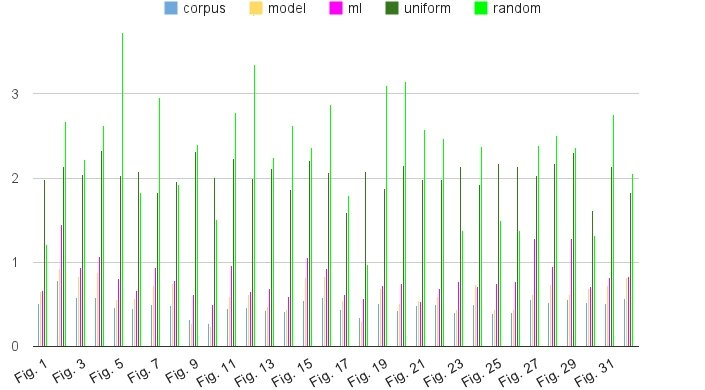
\includegraphics[width=.9\textwidth]{images/entropyComplete.jpg}
%\end{center}
%\vspace*{-2em}
%\caption{Cross-entropy between the corpus distribution of REs and each algorithm \textit{over the GRE3D7}}\label{Entropy}
%\end{figure}



In the figure at~\ref{sec:apendice} we can observe that the learning and model cross-entropies are, in general, much closer to the corpus entropy than the random and uniform cross-entropies. \textit{In Figures 18 and 30 the random distribution are better and closer to learning and model because the randomly selected values of \puse are close to the learned values of \puse by chance. Those are also evident in Table~\ref{results-algo-all} where random are 31,66\% for Fig. 18 and 38,83\% for Fig. 30.}
In the figure we can also observe that the algorithm that uses the \puse directly calculated on the corpus of the scene (model) has a cross-entropy with respect to the corpus distribution that is very close to the cross-entropy between the corpus distribution and the distribution obtained by the algorithm when run with the \puse learned from corpora that does not describe the target scene (learning). This observation supports the learning mechanism proposed in Section~\ref{subsec:learning} to estimate the \puse when no corpora of REs of the target scene is available. 

\subsection{Evaluation of the TUNA-corpus}
%\label{sec:evaluationTUNA}

In this section we present the comparison of our algorithm to the state of the art algorithm Graph introduced above. The Graph algorithm is a deterministic algorithm and hence produces the same referring expression when run with the same target and model. Our algorithm is non deterministic, it may give a different referring expression each time it is run. In order to compare them we run our algorithm k times and we make a ranking of the top 20 produced referring expressions ordered by the frequency they were produced. We use the test part of the TUNA corpus to compare ourselves to the Graph algorithm whose results on this dataset are described in~\cite{KrahmerGRAPH} and reproduced in the Table~\ref{Tabla_sis_1_20}. 

The Graph algorithm defines the generation of referring expressions as a graph search problem, which outputs the cheapest distinguishing graph (if one exists) given a particular cost function. This algorithm is NP-complete in worst-case complexity while our algorithm using the \el language is polynomial. We compare to this algorithm using the metrics accuracy, Dice and \textsc{masi}. Accuracy is defined as the percentage of exact matches between each RE produced by a human and the RE produced by the system for the same scene. 

Dice coefficient is a set comparison metric, ranging between 0 and 1, where
1 indicates a perfect match between sets. For two
attribute sets A and B, Dice is computed as follows:\\

$Dice(A,B) = \frac{2\times|A \cap B|}{|A|+|B|}$\\


The \textsc{masi} score \cite{Passonneau06measuringagreement}~is an adaptation of the Jaccard coefficient
which biases it in favor of similarity where one set
is a subset of the other. Like Dice, it ranges between
0 and 1, where 1 indicates a perfect match. It is computed as follows:\\


$\textsc{masi}(A,B) = \delta \times \frac{|A \cap B|}{|A \cup B|}$ \\


where $\delta$ is a monotonicity coefficient defined as follows:


 \begin{equation}
     \delta  = \left\{
	       \begin{array}{ll}
		 0      & if A \cap B = \emptyset \\
		 1 & if A = B  \\
		 \frac{2}{3}     & if A \subset B ~or~ B \subset A\\
		 \frac{1}{3}     & otherwise
	       \end{array}
	     \right.
 \end{equation}


Intuitively, this
means that those system-produced descriptions are
preferred which do not include attributes that are
omitted by a human.  

In Table~\ref{Tabla_sis_1_20} we show the automatic metrics and compare the performance of our system  with the graph system for the first RE in the ranking and the first 20 REs in the ranking. 

\begin{table}[h!]
\begin{center}
\begin{tabular}{|l|c|c|c|}
\hline
%Figure & Model \puse &  Learning \puse & Random \puse &  Uniform \puse \\
	 	& 	Dice		&	\textsc{masi}	&	ACCURACY		\\
\hline
GRAPH system, Furniture domain	& 	.80 		&	.59	&	.48		 	\\
GRAPH system, People domain 	& 	.72		&	.48	&	.28			\\
\hline
Our system, Furniture domain (top 1)	&	.80		&	.60	&	.47		\\
Our system, People domain (top 1)	&	.65		&	.37	&	.19		\\
\hline
Our system, Furniture domain (top 20)&	.87		&	.75  	&	.65		\\
Our system, People domain (top 20)   &	.81		&	.68	&	.60		\\
\hline
\end{tabular}
%\vspace*{.1cm}
\caption{Comparison of the Graph algorithm and our system. We consider the 3 automatic metrics for the top 1 and the top 20 REs produced by our algorithm.}
\vspace*{-.5cm}
\label{Tabla_sis_1_20}
\end{center}
\end{table}
%\vspace*{-.9cm}
%Estos son los numeros que obtuve de accuracy para furniture (con estos hice el grafico)
%	GRAPH	OUR SYSTEM
%1	0.48	0.43
%5	0.48	0.5
%10	0.48	0.5375
%15	0.48	0.6
%20	0.48	0.65

% y estos para people
%	GRAPH	OUR SYSTEM
%1	0.28	0.19
%5	0.28	0.42
%10	0.28	0.47
%15	0.28	0.54
%20	0.28	0.6

Accuracy, Dice and \textsc{masi} assess humanlikeness with respect to a corpus of human referring expressions. In the Figure~\ref{graficoPresicion} the accuracy for our system and the graph system is compared. The left graph corresponds to the furniture domain and the right graph corresponds to the people domain. We can see that taking the top 1 RE our system accuracy is lower than Graph performance for the people domain. However, if we consider the top 20 REs that our algorithm is able to produce we can see that the accuracy for both domains gets higher than 60\%. This shows that our algorithm is able to generate REs that are more similar to those produced by humans than the graph algorithm, although these REs are not ranked first. 

Another result that we can observe is that the people domain accuracy is much lower for the top 1 RE than for the furniture domain (19 vs 46), but the accuracy stabilizes when REs lower in our ranking are considered. This may be explained by the fact that the training set for the people domain is smaller and less balanced and hence, the probabilities of use inferred do not generalize as well as in the furniture domain. 

\begin{figure}[ht]
\begin{minipage}{0.49\linewidth}
\centering
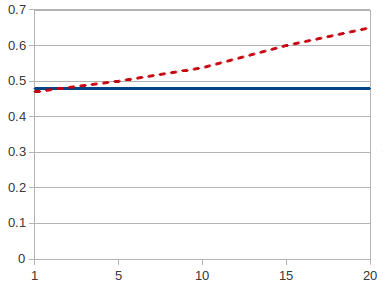
\includegraphics[width=\textwidth]{images/furniturePrec.png}
%\end{figure}
\end{minipage}
%\begin{figure}[ht]
\begin{minipage}{0.49\linewidth}
\centering
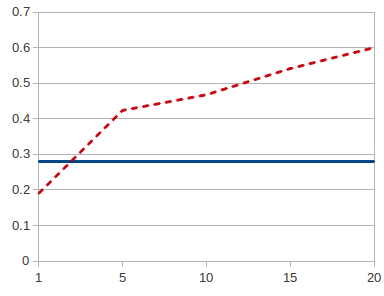
\includegraphics[width=\textwidth]{images/precP.png}
\end{minipage}
\caption{Comparison of the accuracy of the Graph algorithm and our system. The x axis shows indicates that the accuracy was calculated considering the x first REs in the ranking. The y axis indicates the accuracy. Our system is depicted as a dotted line and the Graph system as a continuous line.\label{graficoPresicion}}
\end{figure}

 

%The dotted line is that represented by our system and the another is that represents the GRAPH performance.

%Also we analyze the RE founded in the corpus that the system does not generate in a first frequency, and found that there were a 13.75\% in furniture that were not RE, those were underspecified sentences with does not identifies the target object. For people the proportion was lower just a 5.88\%. We saw that when a person used another word that was not taking into account in the annotation of the corpus, it was annotated as ``other'', and our system was not capable of generate ``other'' because it was not in the model.
%In the table~\ref{error-furniture} there is a percentage of times in 100 runs that the system does not generates the RE given by the human for furniture, and as showed in Table~\ref{error-people} the human were more difficult to generate in the first 100 because the RE were longer the RE have less probability of occur. If the system does not generates the RE in 100 of runs does not mean that the system could not generate them, it just mean that the system need to be running more in order to generate this RE.\\


%\begin{table}[h!]
%\begin{center}
%\begin{tabular}{|l|c|c|}
%\hline
%		& Count		& Percentage\\
%\hline
%It is not RE	&	11	&	13.75 \\
%%		&	37	&	46.25\% \\
%Contains ``other''	&	6	&	7.50 \\
%\hline
%SYS does not generated the RE in 100 runs	&	8	&	10.00 \\
%SYS generated but not with higher frequency	&	18	&	22.5 \\
%\hline
%\end{tabular}
%%\vspace*{.1cm}
%\caption{Clasification of RE that the system could not generates or generates with low frequency for Furniture}
%\label{error-people}
%\end{center}
%\end{table}
%%\vspace*{-.4cm}

%\begin{table}[h!]
%\begin{center}
%\begin{tabular}{|l|c|c|}
%\hline
%			& Count		& Percentage\\
%\hline
%It is not RE		&	4	&	5.88 \\
%Contains ``other''	&	6	&	8.82 \\
%\hline
%SYS does not generated the RE in 100 runs	&	17	&	25.00 \\
%SYS generated but not with higher frequency	&	28	&	41.18 \\
%%BIEN			&	13	&	19.12\% \\

%\hline
%\end{tabular}
%%\vspace*{.1cm}
%\caption{Clasification of RE that the system could not generates or generates with low frequency for People}
%\label{error-furniture}
%\end{center}
%\end{table}
%%\vspace*{-.4cm}

\subsection{Human evaluation} \label{sec:humanevaluation}

We asked two human judges native speakers of English to evaluate our referring expressions via an experiment on the web. The authors of the paper did not participate during the evaluation. The judges could register to the evaluation system so that they did not have to complete it in one go, the could come back to it later. During the evaluation we showed each judge the scenes and two randomly ordered REs. One RE corresponded to the RE present in the corpus and produced by a person and the other RE corresponded to the top 1 RE produced by our system. We asked the judges to select the RE that would be more useful to identify the target in the scene. That is, to select it from among the other objects in the stimulus pictures. 

Our goal is to show that even if the RE generated by our algorithm does not coincide with the RE produced by a human in the corpus collection, it can be judged as good or even better than the REs generated by humans. 

%\begin{table}[h!]
%\begin{center}
%\begin{tabular}{|c|c|c|c|}
%\hline
%           & Agree in & Not agree & Total\\
%\hline 
%Furniture & 25       & 18        & 43 \\
%People    & 25       & 30        & 55 \\
%Total     & 50       & 48        & 98 \\
%\hline
%\end{tabular}
%\caption{Agree between judges} 
%\label{agree-judges}
%\end{center}
%\end{table}

%esta tabla no ayuda...no se que decir, no se como justificar que no coincidan...
%In the Table~\ref{agree-judges} we can see that the both judges choice the same RE 25 times for Furniture and 25 times for People, 

In Table~\ref{system-versus-human} we show the results from the human evaluation experiment.
The REs produced by the system were considered equal or better by both
judges in 60 \% of the cases and, by at least one judge in 92\% of the cases.

\begin{table}[h!]
\begin{center}
\begin{tabular}{|l|c|c|c|c|}
\hline
%total scenes in evaluation set &                           80   &             68
 & Furniture domain & People domain & Weighted mean \\
\hline
system equal to human  	&	.46	&	.19	&	.33 \\
system better by 2 judges &	.29 	& 	.24 	& 	.27 \\
system better by 1 or 2 judges & .51	&	.68	&	.59 \\
system worse by 2 judges &	.03	&	.13	&	.08 \\
system equal or better by 2 judges  &.75  &       .43	&       .60 \\
system equal or better by 1 judge  &.97	&	.87	&	.92 \\
\hline
\end{tabular}
%\vspace*{.1cm}
\caption{Percentage of system versus human selected choices} 
\label{system-versus-human}
\vspace*{-.5cm}
\end{center}
\end{table}

%In the Table~\ref{system-versus-human} we show the percentage of the judges selections, the judge selected more the RE generated by our system than the human RE.

%\begin{table}[h!]
%\begin{center}
%\begin{tabular}{|c|c|c|c|}
%\hline
%Judge    & Human choice & System choice & Total\\
%\hline 
%Judge1 & 25       & 30        & 55 \\
%Judge2    & 23       & 32        & 55 \\
%\hline
%\end{tabular}
%\caption{System versus human selected choice for People} 
%\label{system-versus-human-people}
%\end{center}
%\end{table}

%In the case of pictures of people you can see in the Table~\ref{system-versus-human-people} that the judges selected more RE generated by our system but the difference in not very significant.

%\begin{table}[h!]
%\begin{center}
%\begin{tabular}{|c|c|c|c|c|c|}
%\hline
%           & System & System (\%) & Human & Human (\%) & Total\\
%\hline
%Furniture & 23  & .92 &  2 & .08  & 25 \\
%People    & 16  & .64 & 9  & .36 & 25 \\
%\hline
%Total     & 39  & .78    & 11 & .22 & 50  \\
%\hline
%\end{tabular}
%%\vspace*{.1cm}
%\caption{Coincidences between judges, the system is the preferred the 78\% of times} 
%\label{system-better}
%\end{center}
%\end{table}
%%\vspace*{-.9cm}
%Taking into account just the coincidences between judges the Table~\ref{system-better} shows the percentage of their preference, they preferred the system in 78\% of times.

%Sometimes comparison was unfair because human gives a RE that includes relation that were not annotated so, the system haven't the possibility of produce them. A point in favor of the system is that sometimes the human did an underspecified RE and the system has a better one.

Below, we illustrate the evaluation experiment by showing examples of cases in which the system expression was considered better by both judges, by only one judge or by neither of them. 

Figure~\ref{smallBlueFan} illustrates a case in which the human generated an underspecified RE while the system produced an RE which univocally identifies the target. The RE generated by the system for this figure is ``small blue fan'' while the RE produced by the human is ``blue fan''. The human RE fails to uniquely identify the target and is then not preferred by the human judges. Humans are known for producing underspecified REs which may be due to cognitive limitations for not being able to consider the whole referential context at the same time. Our algorithm is able to consider the whole referential context and combine this ability with the probability of use of the REs learned from humans. 

\begin{figure}[h]
\begin{minipage}{0.49\linewidth}
\centering
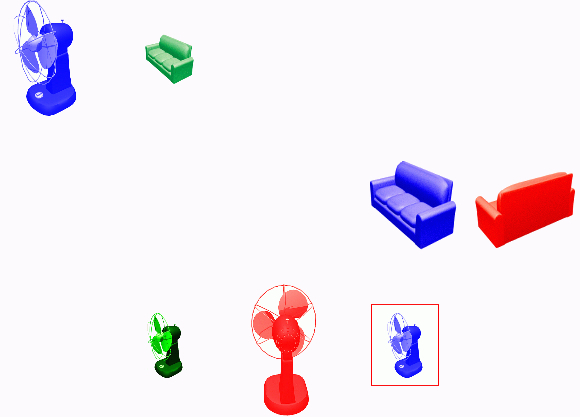
\includegraphics[width=\textwidth]{images/smallBlueFan.jpg}
\caption{Scene used during the collection of the TUNA corpus. The human RE \emph{blue fan}, and the system \emph{small blue fan}. Judges prefer the system generated.}
\label{smallBlueFan}
\end{minipage}
\begin{minipage}{0.49\linewidth}
\centering
\vspace*{.4cm}
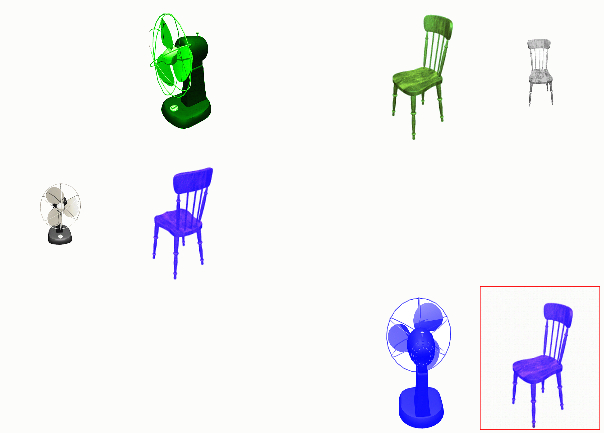
\includegraphics[width=\textwidth]{images/tuna.jpg} % esta es la 101t5 la que mostramos al principio
\vspace*{-.4cm}
\caption{Scene used during the collection of the TUNA corpus. The human RE was \emph{blue frontal chair}, and the system \emph{the blue chair in the bottom}. Both human judges prefer the system generated RE.}
\label{BlueChair}
\end{minipage}
\end{figure}


In Figure~\ref{BlueChair} the human RE was ``blue frontal chair'', and the system RE was ``the blue chair in the bottom''; both judges selected the system RE. This case can be explained by the fact that, in this domain, the property ``bottom'' helps more during the identification than the property ``frontal'' because it concentrates the attention of the interpreter in the lower part of the scene. Our system learns this fact by learning a higher value of \puse~for ``bottom'' than for ``frontal'' from the training data. 

%Sometimes the judges choice the human RE for example in Figure~\ref{largeGreyChair} the
%system RE was ``large grey chair facing away'' and the human RE was ``the top left grey chair''.

%\begin{figure}[ht]
%%\begin{minipage}{0.50\linewidth}
%\centering
%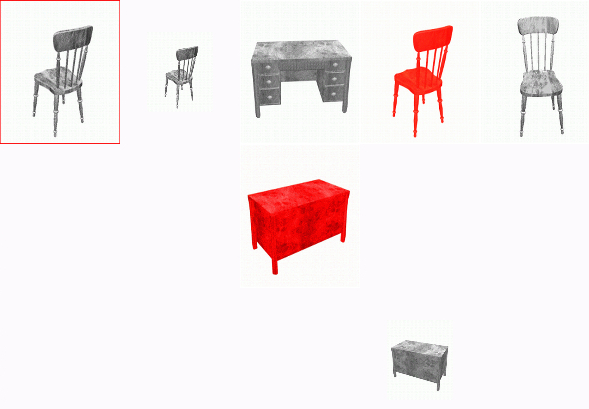
\includegraphics[width=0.8\textwidth]{images/largeGreyChair.jpg}
%\caption{TUNA corpus furniture scene}
%\label{largeGreyChair}
%\end{figure}

\begin{figure}[h]
\begin{minipage}{0.49\linewidth}
\centering
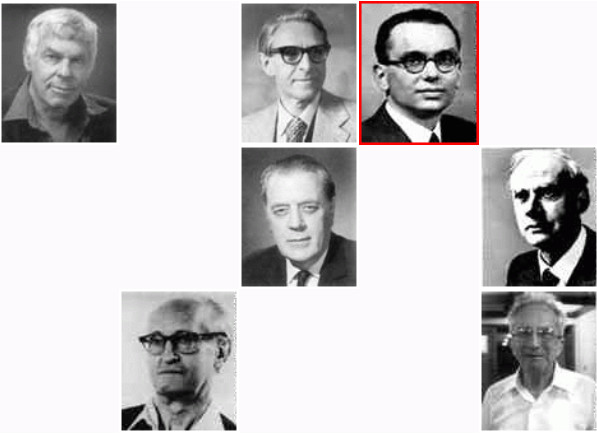
\includegraphics[width=\textwidth]{images/s59t26.jpg}
\caption{Scene used during the collection of the TUNA corpus. The human  RE was \emph{the man with black hair}, and the system \emph{the man wearing glasses in the fourth column}. Judges prefer the human RE.}
\label{s28t25}
%\end{figure}
\end{minipage}
%\begin{figure}[ht]
\begin{minipage}{0.49\linewidth}
\centering
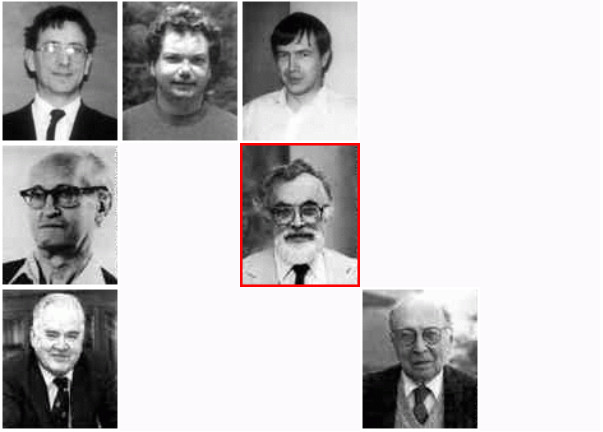
\includegraphics[width=\textwidth]{images/s315t21.jpg}
\vspace*{-.3cm}
\caption{Scene used during the collection of the TUNA corpus. The human RE was \emph{man with a beard}, and the system \emph{man with a beard wearing glasses}. Judges did not agree in their preference.}
\label{s307t21}
\end{minipage}
\end{figure}

Figure~\ref{s28t25} is an example for which both judges preferred the human expression. The human  RE was ``the man with black hair'', and the system's ``the man wearing glasses in the fourth column''. This example makes evident the fact that, in the people domain some properties are more salient in some images than in others because of different shades of colours. Gradable properties such as this ones (in contrast to absolute properties) are still an open problem for GRE algorithms. 

Figure~\ref{s307t21}~illustrates a case in which the system RE was more overspecified than the human RE; the system included ``wearing glasses'' while the human did not. In this case one human subject preferred the system RE and the other the human RE. The amount of overspecification is a subjective matter where human themselves disagree. Further evaluation where REs are actually used for a task would be interesting to investigate this issue.  


